\documentclass[paper=a4,12pt,titlepage,listof=totoc,index=totoc,bibliography=totoc]{scrartcl}
\usepackage[english]{babel}
\usepackage[T1]{fontenc}
\usepackage[english]{translator}
\usepackage{graphicx}    % zur Einbindung von Bilddateien
\usepackage{scrpage2}    % notwendig um z.B. Kopfzeile zu definieren
\usepackage{subfig}      % mehrere Bilder nebeneinander
\usepackage{psfrag}
\usepackage[numbers]{natbib}   % anstelle von cite, bessere Zitier-Moeglichkeiten
\usepackage{amsmath}
\usepackage[numbers]{natbib}
\usepackage{float}

\begin{document}

\section{Rankine-Hugoniot Bedingung}

Ich werde eine kurze Herleitung der Rankine-Hugoniot Bedingung vorstellen.\\
Ausgangspunkt sind die dreidimensionalen instation\"aren Eulergleichungen in konservativer Form:
\begin{equation}
Q_{t}+F_{x}+G_{y}+H_{z}=0.
\label{eq:Euler}
\end{equation}
Die linke Seite kann als Divergenz eines vierdimensionalen Vektors gesehen werden und \"uber Raum und Zeit integriert werden
\begin{equation}
\int_{V_+}^{} \!  \nabla . \left(
 \begin{array}{ccc}
Q \\ F \\ G \\ H
\end{array} \right)\ \mathrm{d} V_+ =0,
\end{equation}\\
wobei $\mathrm{d} V_+=\mathrm{d}x \mathrm{d}y \mathrm{d}z \mathrm{d}t$ und $\nabla=\left(
 \begin{array}{ccc}\partial{}/\partial{t}\\ \partial{}/\partial{x} \\ \partial{}/\partial{y}\\ \partial{}/\partial{z} \end{array} \right)$ ist.\\
Durch Anwendung des Gau\ss-Theorems erh\"alt man dann:\\
\begin{equation}
\int_{A_+}^{} \!   \left(
 \begin{array}{ccc}
Q \\ F \\ G \\ H
\end{array} \right)\ . \overrightarrow{n} \mathrm{d} A_+ =0,
\end{equation}
mit $\mathrm{d} A_+$ dem Oberfl\"achenelement von $\mathrm{d} V_+$ und dem dazugeh\"origen Normalenvektor $\overrightarrow{n}$.\\
Wenn man sich nun eine Diskontinuit\"at in Raum und Zeit vorstellt und \"uber ein Kontrollvolumen das durch diese in zwei Kontrollvolumina eins was wir mit $V_+^R$ und eins was mit $V_+^L$ bezeichnen wollen getrennt wird integriert und dabei vor Augen h\"alt dass  ausserhalb der Diskontinuit\"at der Integrand verschwindet:\\
\begin{equation}
\Delta^{L,R} \int_{A_+^{disk}}^{} \!   \left(
 \begin{array}{ccc}
Q \\ F \\ G \\ H
\end{array} \right)\ . \overrightarrow{n} \mathrm{d} A_+ =0.
\end{equation}\\
Wenn man zus\"atzlich ber\"ucksichtigt dass die Kontrollvolumina bzw. deren Fl\"ache entlang der Diskontinuit\"at beliebig gross gew\"alt werden k\"onnen so erh\"alt man dass der Sprung \"uber die Diskontinuit\"at verschwinden muss:\\
\begin{equation}
\Delta^{L,R} \left[ \left(
 \begin{array}{ccc}
Q \\ F \\ G \\ H
\end{array} \right)\ . \overrightarrow{n} \right] =0.
\label{final}
\end{equation}\\
Die Diskontinuit\"at bewege sich nun mit der Geschwindigkeit $\overrightarrow{c}=\left(c_x,c_y,c_z\right)^T$ dann ist $n_t=-\left(c_x n_x+c_y n_y+c_z n_z\right)$.\\
Und somit kann Gleichung (\ref{final}) geschrieben werden als\\
\begin{equation}
\Delta^{L,R} \left[-Q\left(c_x n_x+c_y n_y+c_z n_z\right) +F n_x+G n_y+H n_z\right] =0,
\end{equation}\\
was das gleiche ist wie\\
\begin{equation}
\Delta^{L,R} \left[ -Q \overrightarrow{c} .
\left( \begin{array}{ccc}
n_x \\ n_y \\ n_z
\end{array} \right)+ \left(
\begin{array}{ccc}
F \\ G \\ H
\end{array} \right).
\left( \begin{array}{ccc}
n_x \\ n_y \\ n_z
\end{array} \right) \right] = 0.
\end{equation}\\
\begin{figure}[H]
\centering
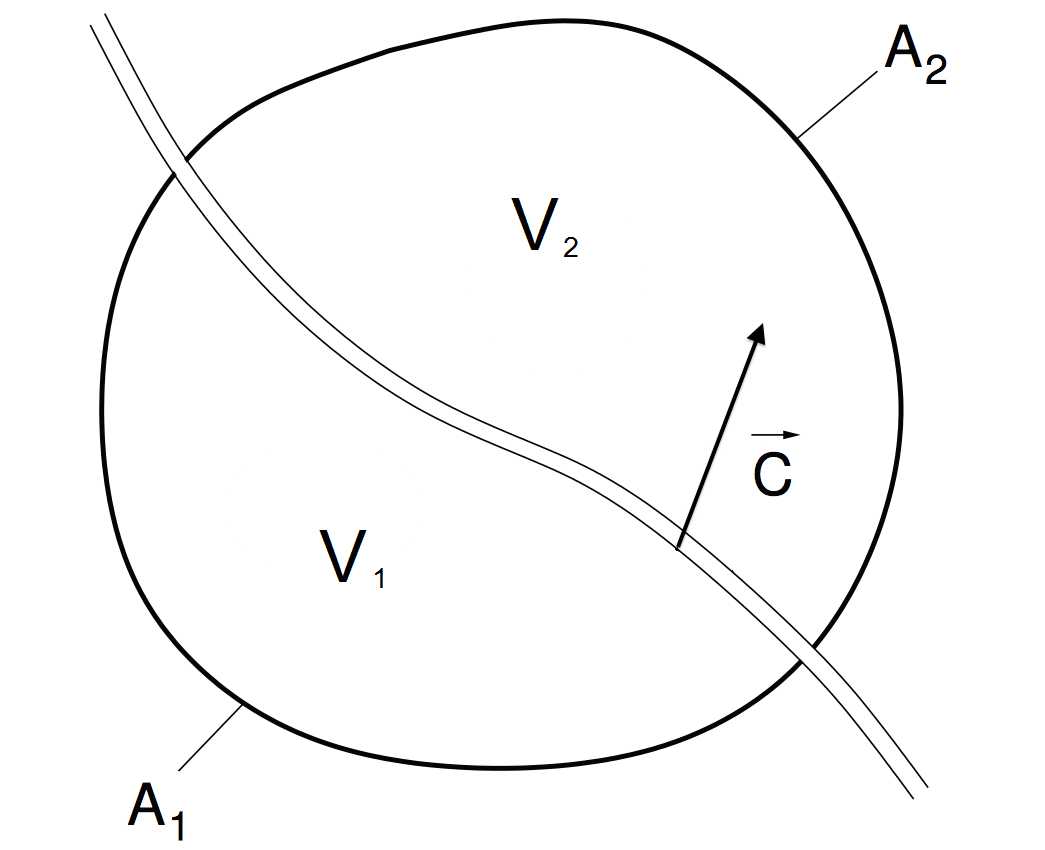
\includegraphics[trim=0cm 0cm 0cm 0cm,clip,  width=0.72\textwidth]{figures/Disk.png}
\caption{Diskontinuit\"at und Kontrollvolumina.}
\label{fig:Disk}
\end{figure}
\end{document}
